\chapter{Modelos de neurônio de disparo}\label{cap:modelos}
\section{Introdução}\label{sec:modelos_intro}
Os modelos são formas de representar, matemática e/ou computacionalmente, o comportamento do neurônio. Os modelos podem variar desde os mais simples, que não representam fielmente o comportamento fisiológico do neurônio mas são úteis para simular grandes quantidades de neurônios, até os mais complexos, que trazem diversas representações de condutância e morfológicas. Alguns modelos de neurônio são apresentados na Tabela~\ref{tab:modelos_neuronios}, incluindo o número de variáveis presentes no modelo, o que reflete o número de equações diferenciais presentes e, consequentemente, a complexidade do mesmo, bem como é informado se o modelo é considerado biologicamente plausível. Os 4~(quatro) primeiros modelos são detalhados neste texto, por hora diferenciados entre os que simulam o disparo do potencial de ação, chamados aqui de modelos de neurônio de disparo, e os que simulam a taxa de disparo, detalhados no Capítulo seguinte. Há, ainda, distinção, por exemplo, entre modelos de compartimento único, que modelam o potencial de membrana apenas pela variável $V$, e os multi-compartimento, que consideram variações espaciais no potencial de membrana, porém estes últimos não são abordados neste texto.

\begin{table}
	\IBGEtab{
	\centering
	\caption[Modelos de neurônio]{Modelos de neurônio}
	\label{tab:modelos_neuronios}
	}{
	\begin{tabular}{|c|c|c|c|}
		\hline
		Modelo & N. variáveis & Complexidade & Biol. plausível \\
		\hline
		Leaky integrate-and-fire & 1 & Muito baixa & Não \\
		\hline
		Izhikevich & 2 & Muito baixa & Não \\
		\hline
		Hodgkin-Huxley & 4 & Muito alta & Sim \\
		\hline
		Wilson-Cowan & 2 & Média & Não \\
		\hline
		Spike response model & 1 & Baixa & Não \\
		\hline
		FitzHugh-Nagumo & 2 & Média & Não \\
		\hline
		Moris-Lecar & 3 & Alta & Sim \\
		\hline
	\end{tabular}
}{
\fonte{O autor (2023)}
}
\end{table}

\section{Modelo integra-e-dispara com vazamento}\label{sec:modelolif}

Para modelos de neurônio de compartimento único, o circuito elétrico equivalente da membrana pode ser representado como na Figura~\ref{fig:circuitomembrana}.
\begin{figure}[htb!]
	\centering
	\caption{Circuito equivalente da membrana}
	\label{fig:circuitomembrana}
	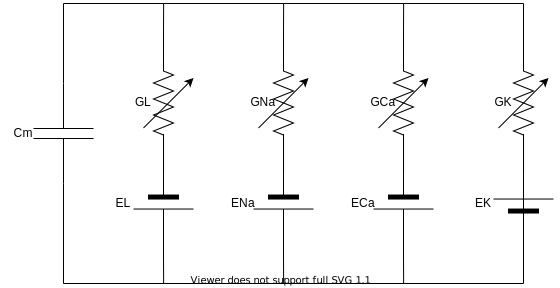
\includegraphics[width=0.7\linewidth]{figs/circuito_membrana}
	\fonte{O autor (\the\year)}
\end{figure}
O capacitor na esquerda está associado à capacitância da membrana ($C_m$), e cada resistor em série com uma bateria representa um canal iônico. A série com o $L$ subscrito refere-se ao elemento de vazamento, citado anteriormente, e as séries são referentes aos canais iônicos dependentes de tensão, com o íon subscrito. O circuito completo tem associada a seguinte equação:
\begin{equation}\label{eq:potencial_membrana_total}
	c_m\frac{\mathrm{d}V_m}{\mathrm{d}t}=G_{Na}(E_{Na}-V_m)+G_{Ca}(E_{Ca}-Vm)+G_K(E_K-V_m)+G_L(E_L-V_m)
\end{equation}
sendo $G_A$ a condutância do íon $A$, $E_A$ o potencial do íon $A$. Ignorando por hora os canais iônicos dependentes de tensão, a equação fica como a \ref{eq:potencial_membrana}. Adicionando-se a corrente aplicada, incluímos também uma condição que força o disparo do potencial de ação quando o potencial de membrana atinge um determinado limitar ($V_{th}$), forçando o potencial de membrana para um valor de \textit{reset} ($V_{reset}$) \cite{miller_introductory_2018}. Com isso, o circuito fica equivalente à Figura~\ref{fig:circuitolif} e a equação total é como abaixo.
\begin{equation}\label{eq:lif}
	c_m\frac{dV_m}{dt} = G_L(E_L-V_m)+I_{ap}; \text{ se } V_m > V_{th} \text{ então } V_m\mapsto V_{reset}
\end{equation}
\begin{figure}[htb!]
	\centering
	\caption{Circuito equivalente do modelo LIF}
	\label{fig:circuitolif}
	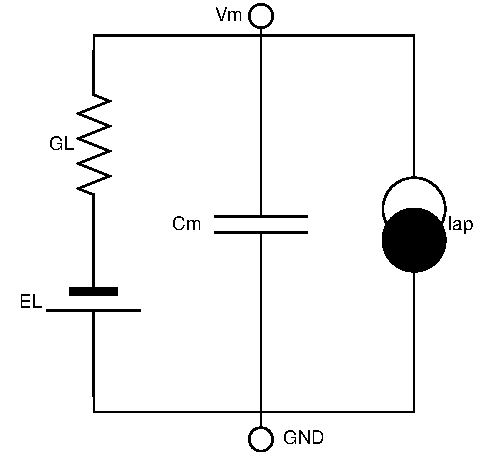
\includegraphics[width=0.5\linewidth]{figs/circuito_lif}
	\fonte{O autor (\the\year)}
	%TODO: trocar GND
\end{figure}
Essa é a equação do modelo \textit{Leaky integrate-and-fire} (LIF, integra e dispara com vazamento, em tradução livre) \cite{lapicque_recherches_1907}. A corrente aplicada no modelo é acumulada (integrada), elevando o potencial de membrana até o valor de limiar, representando o momento onde o neurônio dispara. Devido a simplicidade do modelo, a equação, por si só, não é capaz de representar a hiperpolarização que ocorre fisicamente na célula neuronal após o disparo do potencial de ação, e, por isso, é acrescentada a condição de \textit{reset}. Enquanto a corrente continuar sendo aplicada, o potencial de membrana permanece sendo atualizado pela dinâmica da equação diferencial, como é exibido na Figura~\ref{fig:lif}. Três pulsos de corrente, com valores $0,18\ nA$, $0,21\ nA$ e $0,24\ nA$, são aplicados no modelo. Para o primeiro valor, o neurônio despolariza (fica menos negativo), porém não atinge o valor de limiar (como visto na primeira curva da segunda linha de gráficos). Com a injeção dos demais valores de corrente, a célula neuronal atinge o valor de limiar ($50\ mV$ nestes exemplos), ocorrendo o disparo do potencial de ação (registrado como uma linha vertical na última linha de gráficos), e com a posterior alteração do potencial de membrana para o valor de \textit{reset} ($80\ mV$ nestes exemplos).

\begin{figure}[htb!]
	\centering
	\caption[Exemplo da simulação com o modelo LIF]{Exemplo da simulação com o modelo LIF}
	\label{fig:lif}
	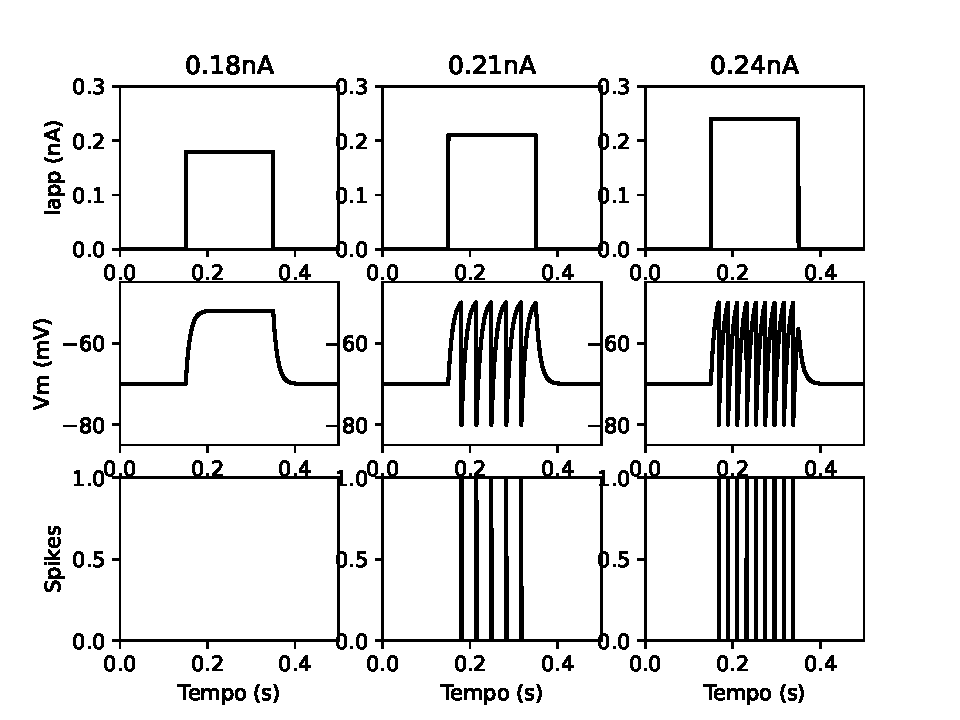
\includegraphics[width=0.7\linewidth]{figs/lif}
	\fonte{O autor (\the\year)}
	%TODO: regerar
\end{figure}

%% incluir a solução analítica para enfatizar a presença da constante de tempo

\subsection{Extensões do modelo LIF}
Apesar de útil e ser utilizado em inúmeras simulações neuronais, o modelo LIF é carente de diversos comportamentos presentes fisiologicamente no neurônio. Algumas delas são apresentadas aqui como extensões ao modelo, a fim de acrescentar algumas características que podem ser úteis nas simulações. As extensões apresentadas simulam a refratariedade e a adaptação da taxa de disparo, além de versões do modelo LIF com componentes exponenciais e adaptativas, como mostradas na sequência.
\subsubsection{Período refratário}
Imediatamente após a ocorrência do potencial de ação, o neurônio não é capaz de produzir um novo potencial de ação durante um curto período de tempo, e esse tempo é chamado de período refratário. Existem diferentes métodos para simular esse comportamento nos modelos neuronais, e aqui mostramos três, acrescentadas ao modelo LIF, com os seus comportamentos exibidos na Figura~\ref{fig:lifrefratario}.
\begin{figure}[tb]
	\centering
	\caption{Simulação do modelo LIF com período refratário}
	\label{fig:lifrefratario}
	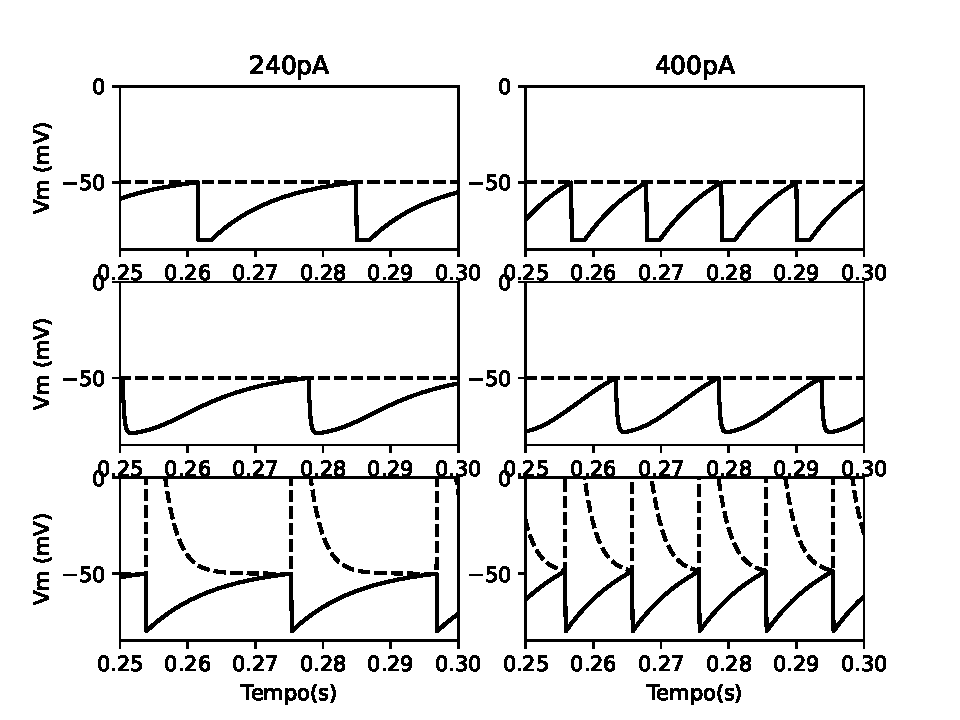
\includegraphics[width=0.7\linewidth]{figs/lif_refratario}
	\fonte{O autor (\the\year)}
	%TODO: regerar
\end{figure}
Em todos os métodos são simuladas a injeção de corrente de $240\ pA$ (primeira coluna de gráficos) e $400\ pA$ (segunda coluna), e a linha tracejada representa o limiar para disparo do potencial de ação. O primeiro método é chamado de \textbf{grampeamento de tensão},que consiste em fixar o potencial de membrana no valor de \textit{reset} durante um tempo específico logo após o potencial de ação. É, provavelmente, a maneira mais simples de simular a refratariedade, pois neste método o período refratário é constante. O segundo método é o da \textbf{condutância refratária}, consistindo no acréscimo de uma condutância elevada, geralmente uma corrente hiperpolarizante de potássio, que cresce imediatamente após a ocorrência de cada potencial de ação, e decai em seguida de acordo com a seguinte equação diferencial:
\begin{equation}\label{eq:condutancia_refrataria}
	\frac{dG_{ref}(t)}{dt} = -\frac{G_{ref}(t)}{\tau_{ref}};\text{ depois do potencial de ação } G_{ref} \mapsto G_{ref} + \Delta G
\end{equation}
sendo $\tau_{ref}$ a constante de tempo do período refratário e $\Delta G$ o incremento de condutância. Como visto na segunda linha de gráficos, o potencial de membrana cresce em um ritmo mais lento que o normal, devido à corrente de potássio que hiperpolariza a célula. Essa corrente é representada acrescentando-se à parte direita da equação do modelo LIF o termo $G_{ref}(t)[E_k-V_m(t)]$, com $E_k$ sendo o potencial de reversão para os íons de potássio (como na Tabela~\ref{tab:concentracao_nernst}). O último método é chamado de \textbf{incremento do limiar}, onde é elevado, após cada potencial de ação, o limiar necessário para ocorrer um novo disparo. Esse limiar decai conforme a equação:
\begin{equation}\label{eq:incremento_limiar}
	\frac{dV_{th}(t)}{dt} = \frac{V^0_{th}-V_{th}(t)}{\tau_{ref}};\text{ depois do potencial de ação } V_{th} \mapsto V_{th} + \Delta V
\end{equation}
sendo $V^0_{th}$ o potencial de limiar de referência (o valor do limiar em repouso). Como visto na última linha de gráficos, o limiar (linha tracejada) cresce absurdamente após cada disparo de potencial de ação, decaindo logo em seguida, ao contrário do potencial de membrana, que decai e cresce em seguida. 

\subsubsection{Adaptação da taxa de disparos}
Uma característica presente nos neurônios é a sua capacidade de adaptar a frequência em que os disparos de potencial de ação ocorrem, com uma diminuição da taxa logo após o primeiro disparo. Uma fácil percepção da consequência da adaptação da taxa de disparo é a diferença de percepção de cheiros intensos ao longo do tempo, como quando uma pessoa entra com um perfume forte em um elevador. A implementação da adaptação da taxa de disparos é feita de maneira semelhante ao método da condutância refratária apresentada anteriormente, porém com duas diferenças:
\begin{itemize}
	\item O incremento da condutância é menor em comparação ao do período refratário. Esse incremento menor não impede o disparo de novos potenciais (o que acontece no período refratário), porém diminui a taxa deles
	\item A escala de tempo (a constante) da condutância adaptativa é bem maior, o que permite o acúmulo das condutâncias ao longo da sequência de disparos
\end{itemize}
A dinâmica da adaptação da taxa de disparos é exibida na Figura~\ref{fig:lifatd}. Como no exemplo do período refratário, correntes de $240\ pA$ e $400\ pA$ são injetadas, sendo exibidas as curvas de potencial de membrana (em cima), e da condutância adaptativa (embaixo), onde se pode observar incremento e acúmulo de condutância.

\begin{figure}[tb]
	\centering
	\caption{Adaptação da taxa de disparo no neurônio LIF}
	\label{fig:lifatd}
	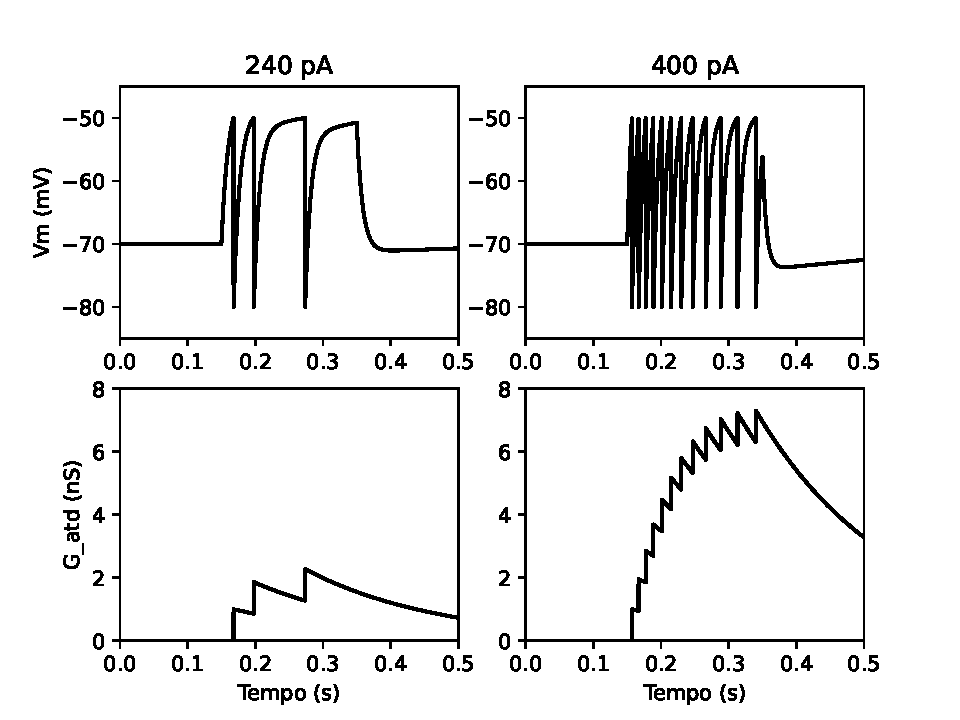
\includegraphics[width=0.7\linewidth]{figs/lif_atd}
	\fonte{O autor (\the\year)}
	%TODO: regerar
\end{figure}

\subsubsection{Modelo LIF exponencial}
O modelo LIF exponencial (\textit{exponential leaky integrate-and-fire}, ELIF, em inglês) incorpora um termo adicional para a geração do potencial de ação, que é uma falta existente no modelo tradicional. Esse termo acrescenta uma corrente despolarizante, elevando quase que instantaneamente o valor do potencial de membrana quando este se aproxima do limiar. Esse crescimento tende ao infinito, porém nas simulações é definido um limite ($V_{max}$), devido o computador ter problemas para lidar com valores infinitos, alterando a condição do modelo para a equação abaixo:
\begin{equation}\label{eq:elif_cond}
	\text{se } V_m > V_{max} \text{ então } V_m\mapsto V_{reset}
\end{equation}
Além disso, não há exatamente um valor fixo para o disparo do potencial, e sim um intervalo ($\Delta_{th}$), e a equação completa deste modelo fica:
\begin{equation}\label{eq:elif}
	c_m\frac{dV_m}{dt} = G_L(E_L-V_m) + G_L\Delta_{th}\exp\Big(\frac{V_m-V_{th}}{\Delta_{th}}\Big) + I_{ap}
\end{equation}
Os gráficos comparando o potencial de membrana do modelo LIF (em cima) e ELIF (embaixo) são mostrados na Figura~\ref{fig:elif}. Uma característica interessante é a inflexão presente no modelo ELIF quando o potencial de membrana se aproxima do instante em que ocorre o disparo do potencial de ação, algo inexistente no modelo LIF.

\begin{figure}[tb]
	\centering
	\caption{Comparação dos modelos LIF e ELIF}
	\label{fig:elif}
	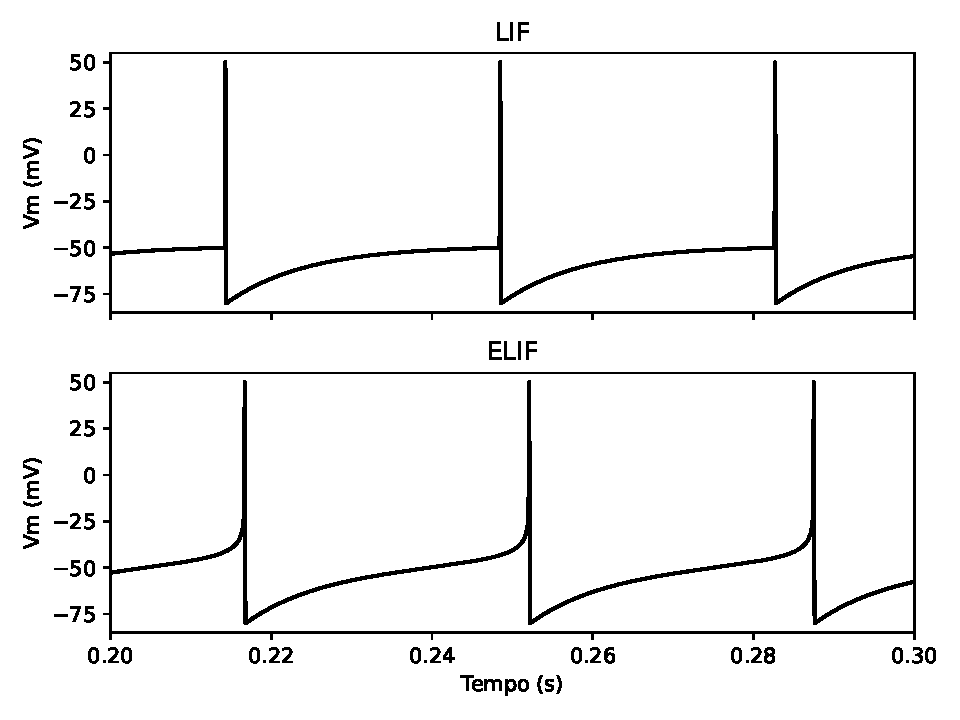
\includegraphics[width=0.7\linewidth]{figs/elif}
	\fonte{O autor (\the\year)}
	%TODO: regerar
\end{figure}

\subsubsection{Modelo LIF exponencial adaptativo}
O modelo LIF exponencial adaptativo (\textit{adaptative exponential leaky integrate-and-fire}, AELIF, em inglês) adiciona uma corrente adaptativa hiperpolarizante ao modelo anterior, similar à utilizada no método da condutância refratária, porém com o decaimento dependendo do potencial de membrana. É um modelo com duas equações, sendo uma para a variável de adaptação ($w$) e a outra para o potencial de membrana, que é semelhante à do modelo anterior, e ambas tem um \textit{reset} quando ocorre o disparo do potencial de ação.
% Esse modelo é capaz de descrever padrões de disparo comuns, como \textit{bursting, fast spiking, regular spiking}, dentre outros.
As equação para este modelo são:
\begin{equation}
	c_m\frac{dV_m}{dt} = G_L(E_L-V_m) + G_L\Delta_{th}\exp\Big(\frac{V_m-V_{th}}{\Delta_{th}}\Big) - w + I_{ap}
\end{equation}
\begin{equation}
	\tau_w\frac{dw}{dt}=a(V_m-E_L)-w
\end{equation}
com as condições:
\begin{equation}
	\text{se } V_m > V_{max} \text{ então } V_m\mapsto V_{reset} \text{ e } w\mapsto w + b
\end{equation}
sendo $a$ o parâmetro de agrupamento, indicando o nível de relação entre o potencial de membrana e a variável de adaptação, e $b$ o parâmetro de adaptação, que é o valor do incremento de corrente após o disparo do potencial de ação. A dinâmica do modelo ELIF é mostrada na Figura~\ref{fig:elif}, com o potencial de membrana exibido em cima e a variável de adaptação embaixo. É possível notar a semelhança da curva de adaptação com a da condutância adaptativa da adaptação da taxa de disparo, também semelhante ao método da condutância refratária.

\begin{figure}[tb]
	\centering
	\caption[Resposta do modelo AELIF]{Resposta do modelo AELIF para um pulso de corrente de 1 $nA$}
	\label{fig:adexrs}
	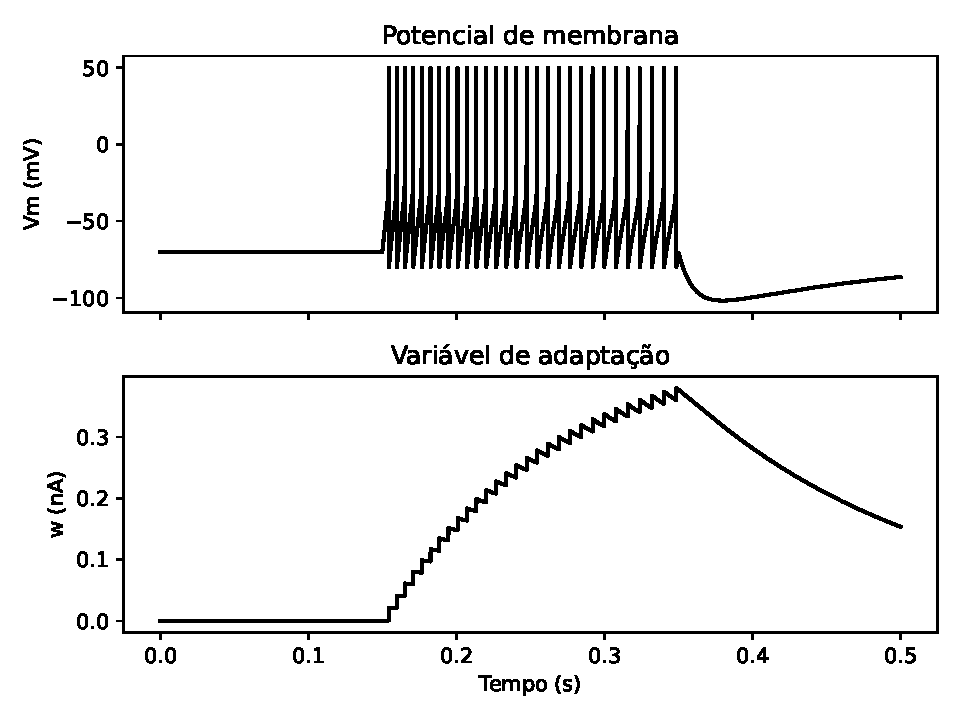
\includegraphics[width=0.7\linewidth]{figs/aelif}
	\fonte{O autor (\the\year)}
	%TODO: regerar
\end{figure}

\section{Modelo de Izhikevich}\label{sec:izhikevich}
Em 2003, Eugene Izhikevich publicou um modelo capaz de simular vários comportamentos de neurônios corticais, combinando a plausabilidade biológica do modelo de Hodgkin-Huxley (que será visto na sequência) com a eficiência computacional do modelo LIF \cite{izhikevich_simple_2003}. Ele é composto por duas equações diferenciais, que são as seguintes:
\begin{equation}\label{eq:izhikevich_v}
	v'=0.04v^2+5v+140-u+I
\end{equation}
\begin{equation}\label{eq:izhikevich_u}
	u'=a(bv-u)
\end{equation}
com as condições de \textit{reset}
\begin{equation}\label{eq:izhikevich_condicao}
	\text{se }v\geq30\ mV,\text{ então }\begin{cases}
		v\leftarrow c\\
		u\leftarrow u+d
	\end{cases}
\end{equation}
com $v$ sendo o potencial de membrana, $u$ a variável de recuperação da membrana, e $I$ sendo a corrente injetada (a notação adotada aqui é a mesma usada por Izhikevich). Na Figura~\ref{fig:izhikevich} é exibido o potencial de membrana para um comportamento do tipo \textit{regular spiking} quando é injetada uma corrente de $10\ mA$.
\begin{figure}[tb]
	\centering
	\caption[Potencial de membrana no modelo de Izhikevich]{Potencial de membrana no modelo de Izhikevich}
	\label{fig:izhikevich}
	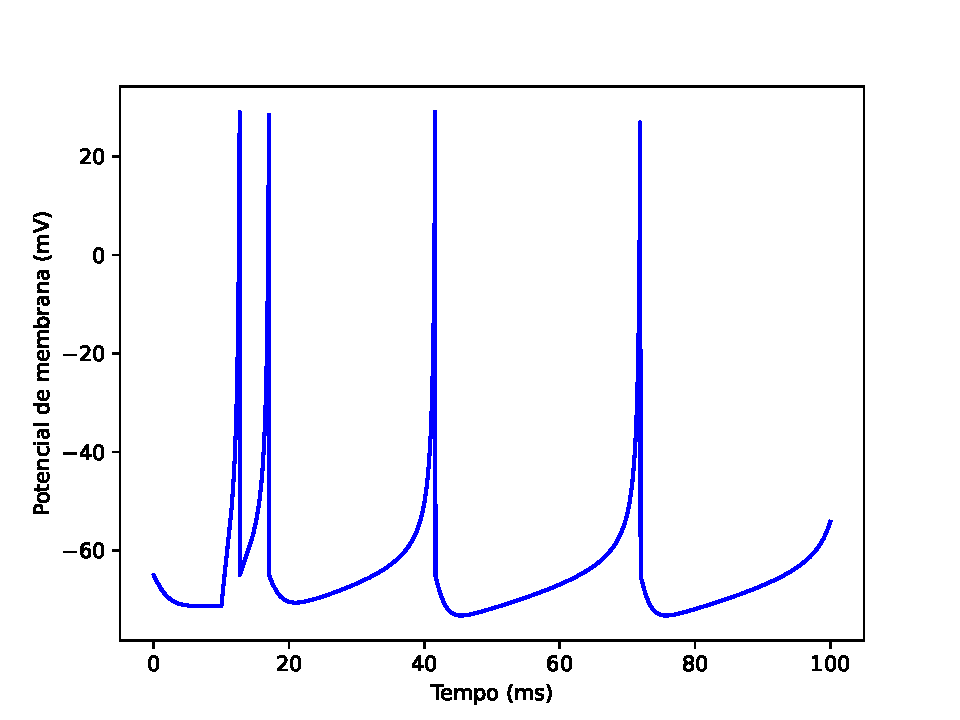
\includegraphics[width=0.7\linewidth]{figs/izhikevich}
	\fonte{O autor (\the\year)}
\end{figure}
Os parâmetros \textit{a}, \textit{b}, \textit{c} e \textit{d} são definidos como segue:
\begin{itemize}
	\item O parâmetro \textit{a} representa a escala de tempo da variável de recuperação, onde valores pequenos resultam em uma recuperação mais lenta
	\item O parâmetro \textit{b} representa a sensibilidade da variável de recuperação às sub-flutuações do potencial de membrana, onde valores maiores agrupam mais $v$ e $u$
	\item O parâmetro \textit{c} representa o valor de \textit{reset} do potencial de membrana após o disparo do potencial de ação
	\item O parâmetro \textit{d} representa o valor de \textit{reset} da variável de recuperação após o disparo do potencial de ação
\end{itemize}
A combinação de determinados valores para os parâmetros acima produz saídas compatíveis com alguns dos comportamentos citados anteriormente, conforme listado na Tabela~\ref{tab:padroes_izhikevich}.
\begin{table}
	\IBGEtab{
	\centering
	\caption[Padrões de neurônio do modelo de Izhikevich]{Padrões de neurônio do modelo de Izhikevich}
	\label{tab:padroes_izhikevich}
	}{
	\begin{tabular}{|c|c|c|c|c|}
		\hline
		Padrão & a & b & c & d \\
		\hline
		\textit{regular spiking} & 0,02 & 0,2 & -65 & 8 \\
		\hline
		\textit{intrinsically bursting} & 0,02 & 0,2 & -55 & 4 \\
		\hline
		\textit{chattering} & 0,02 & 0,2 & -50 & 2 \\
		\hline
		\textit{fast spiking} & 0,1 & 0,2 & -65 & 2 \\
		\hline
		\textit{thalamo-cortical} & 0,02 & 0,25 & -65 & 0,05 \\
		\hline
		\textit{resonator} & 0,1 & 0,25 & -65 & 2 \\
		\hline
		\textit{low-threshold spiking} & 0,02 & 0,25 & -65 & 2 \\
		\hline
	\end{tabular}
}{
	\fonte{O autor, baseado em \cite{izhikevich_simple_2003}}
}
\end{table}

\section{Modelo de Hodgkin-Huxley}\label{sec:modelohh}
O último dos modelos de disparo de neurônio visto neste texto é o de Hodgkin-Huxley \cite{hodgkin_quantitative_1952}. Como visto na Seção~\ref{sec:fisiologia}, existem canais iônicos que são dependentes de tensão. A probabilidade de abertura desses canais é modificada em função do potencial de membrana. O mecanismo de funcionamento deles é como mostrado na Figura~\ref{fig:canais}. À esquerda, é possível ver os elementos que compõem esse tipo de canal: um sensor, que identifica o potencial de membrana; um filtro de seletividade, que seleciona apenas íons compatíveis com aquele canal; e os portões, que permitem ou não a passagem dos íons. Há dois tipos de portões, que estão relacionados aos processos de \textbf{ativação} e \textbf{inativação}. O primeiro refere-se à abertura de um canal iônico, geralmente devido à despolarização, que aumenta a probabilidade de um canal estar aberto. O seu oposto é a \textbf{desativação}, que fecha o canal, geralmente por hiperpolarização. A inativação é o processo que impede a abertura dos canais, tendo como oposto, necessário para que o canal se abra, chamado de \textbf{desinativação}.
\cite{miller_introductory_2018}
\begin{figure}[htb!]
	\centering
	\caption{Mecanismo de funcionamento dos canais iônicos dependentes de tensão}
	\label{fig:canais}
	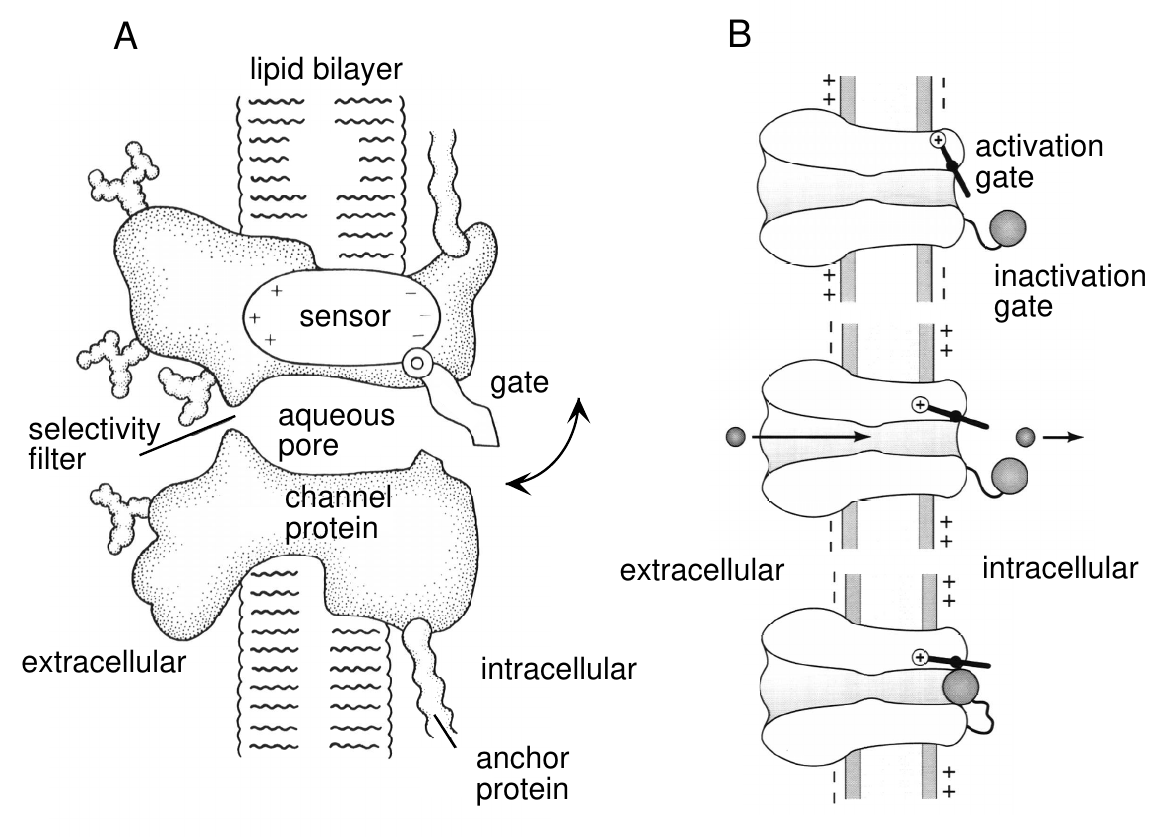
\includegraphics[width=0.6\linewidth]{figs/canais}
	\fonte{\cite{dayan_theoretical_2001}}
	%TODO: trocar figura
\end{figure}
Associado aos canais iônicos dependentes de tensão, existe a chamada \textbf{variável de portão}, que representa a fração desses canais que se encontra em um determinado estado (ativado/desativado, inativado/desinativado). Como se trata da probabilidade do canal estar em um desses estados, seus valores são entre $0$ e $1$. No modelo, são consideradas as variáveis \textbf{m} para ativação de sódio, \textbf{h} para inativação de sódio, e \textbf{n} para ativação de potássio, com as equações a seguir:
\begin{equation}\label{eq:dmdt}
	\frac{dm}{dt}=\alpha_m(1-m)-\beta_mm
\end{equation}
\begin{equation}\label{eq:dhdt}
	\frac{dh}{dt}=\alpha_h(1-h)-\beta_hh
\end{equation}
\begin{equation}\label{eq:dndt}
	\frac{dn}{dt}=\alpha_n(1-n)-\beta_nn
\end{equation}
sendo $\alpha$ a constante de crescimento de cada variável, e $\beta$ a de decrescimento, ambas também dependentes de tensão, conforme as equações abaixo:
\begin{equation}\label{eq:alpha_m}
	\alpha_m=\frac{10^5(-V_m-0.045)}{\exp[100(-V_m-0.045)]-1}
\end{equation}
\begin{equation}\label{eq:beta_m}
	\beta_m=4*10^5\exp\Big[\frac{(-V_m-0.070)}{0.018}\Big]
\end{equation}
\begin{equation}\label{eq:alpha_h}
	\alpha_h=70\exp[50(-V_m-0.070)]
\end{equation}
\begin{equation}\label{eq:beta_h}
	\beta_h=\frac{10^3}{1+\exp[100(-V_m-0.040)]}
\end{equation}
\begin{equation}\label{eq:alpha_n}
	\alpha_n=\frac{10^4(-V_m-0.060)}{\exp[100(-V_m-0.060)]-1}
\end{equation}
\begin{equation}\label{eq:beta_n}
	\beta_n=125\exp\Big[\frac{(-V_m-0.070)}{0.08}\Big]
\end{equation}
\begin{figure}[tb]
	\centering
	\caption{Dinâmica das variáveis de portão}
	\label{fig:portoes}
	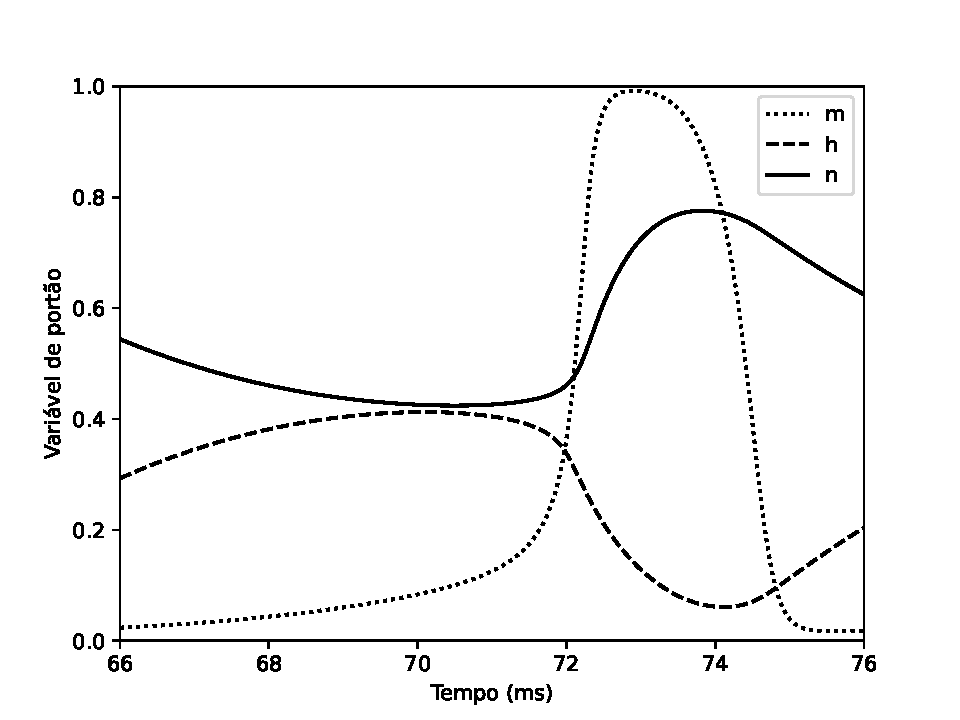
\includegraphics[width=0.7\linewidth]{figs/portoes}
	\fonte{O autor (\the\year)}
	%TODO: regerar
\end{figure}
A dinâmica das variáveis de portão no modelo de Hodgkin-Huxley pode ser vista na Figura~\ref{fig:portoes}, para uma faixa de 66 até $76\ ms$. As variáveis de portão também podem se definidas pelas suas equações em \textbf{regime permanente}, que é o comportamento em repouso depois de um longo período de tempo~\cite{ermentrout_mathematical_2010}, como descritas nas equações abaixo (o símbolo de $\infty$ representa o valor em regime permanente):
\begin{equation}\label{eq:m_inf}
	m_\infty=\frac{\alpha_m}{\alpha_m+\beta_m}
\end{equation}
\begin{equation}\label{eq:h_inf}
	h_\infty=\frac{\alpha_h}{\alpha_h+\beta_h}
\end{equation}
\begin{equation}\label{eq:n_inf}
	n_\infty=\frac{\alpha_n}{\alpha_n+\beta_n}
\end{equation}
com as respectivas constantes de tempo:
\begin{equation}\label{eq:tau_m}
	\tau_m=\frac{1}{\alpha_m+\beta_m}
\end{equation}
\begin{equation}\label{eq:tau_n}
	\tau_h=\frac{1}{\alpha_h+\beta_h}
\end{equation}
\begin{equation}\label{eq:tau_h}
	\tau_n=\frac{1}{\alpha_n+\beta_n}
\end{equation}
Finalmente, o potencial de membrana é dado pela equação abaixo:
\begin{equation}\label{eq:hodgkin_huxley}
	C_m\frac{dV_m}{dt}=G_L(E_L-V_m)+G_{Na}^{(max)}m^3h(E_{Na}-V_m)+G_K^{(max)}n^4(E_K-V_m)+I_{ap}
\end{equation}
que é semelhante à equação do modelo LIF, porém com dois elementos a mais, um para a condutância dependente de tensão de sódio e outra para a de potássio, que incluem as variáveis de portão. O modelo também assume algumas constantes além das usadas em outros modelos, que são a condutância máxima de sódio ($G_{Na}^{(max)}$), a condutância máxima de potássio ($G_K^{(max)}$), o potencial de reversão do sódio ($E_{Na}$) e o potencial de reversão do potássio ($E_K$). A dinâmica do potencial de membrana desse modelo para o mesmo intervalo de tempo é mostrada na Figura~\ref{fig:hhvm}.

\begin{figure}[tb]
	\centering
	\caption{Potencial de membrana gerado pelo modelo de Hodgkin-Huxley}
	\label{fig:hhvm}
	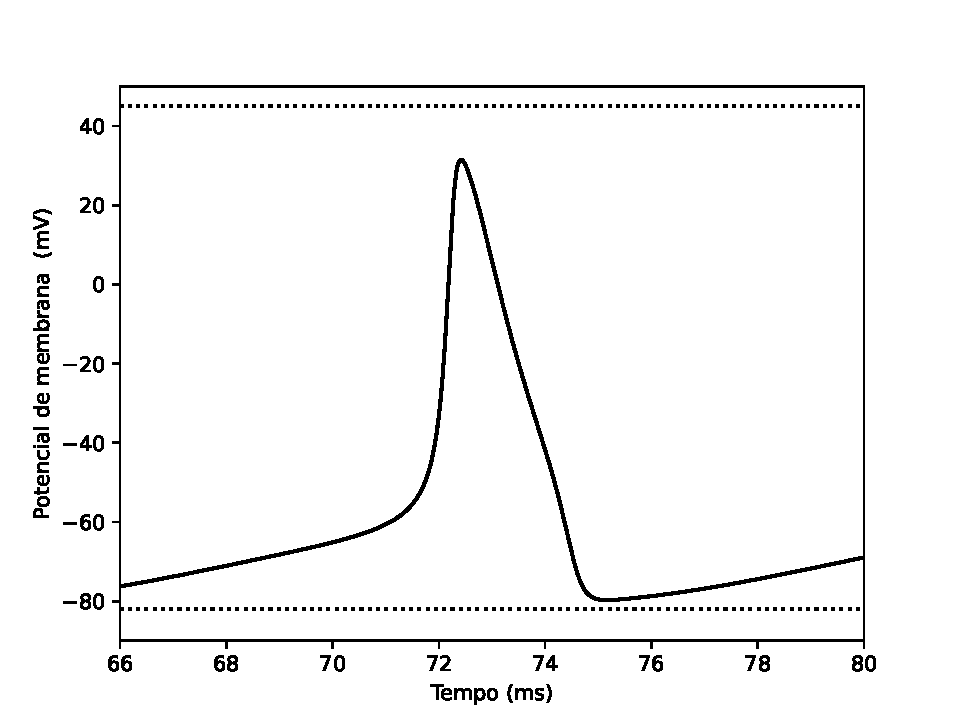
\includegraphics[width=0.7\linewidth]{figs/hh_vm}
	\fonte{O autor (\the\year)}
	%TODO: regerar
\end{figure}
